% !TeX root = ../../main.tex
\section{Ubi-Interact}\label{section:ubi-interact}
\setcounter{footnote}{0} % for some reason, the footnote wants to start at 2

\ac{UBII}\footnote{UBII is currently developed and maintained by Sandro Weber, who is also the advisor for this thesis.} is a framework for distributed applications, which enables to connect all kinds of different devices together. A centralized server is used to manage the system in a local network. The abstraction into devices, topics, and interactions allows decoupling  the implementation of software from device-specific environments.


\subsection{Architecture}\label{subsection:architecture}

The main components of the \ac{UBII} framework are:
\begin{description}
	\item[\ac{UBII} Clients] describe a basic network participant. For every \ac{UBII} client registered on the server also exists one network socket address. Clients are an abstraction of a physical network device. They are defined by a \ac{UID}. 
	\item[\ac{UBII} Devices] can be registered by clients. A \ac{UBII}-device groups different input and output \ac{UBII} devices together. It is defined by a \ac{UID} and a list of \ac{UBII} components.
  \item[\ac{UBII} Components] contain the \ac{UBII} topic name, \ac{UBII} message formats for input/output \ac{UBII} devices and whether it publishes input or receives output data. A data source for such an input \ac{UBII} device, could be any sensor, for example, a button or a camera. Data output examples for input \ac{UBII} devices are lamps and displays.
  \item[\ac{UBII} Message Formats] define the format of data published to a \ac{UBII} topic. Even though it is possible to implement custom ones, most common data types are available. \sloppy{For example, \lstinline[mathescape=true]{Vector4$\times$4} (a four by four matrix), \lstinline{Vector2} (a two-dimensional vector) or \lstinline{boolean} (a binary value) are built-in.} % chktex 46
	\item[\ac{UBII} Topics] are data channels which are addressed by a name. \ac{UBII} Clients can publish messages to \ac{UBII} topics, which are registered by a \ac{UBII} device. They are able to receive messages, after subscribing to a \ac{UBII} topic. Such messages (also called \enquote{\ac{UBII} topic data}) are formatted as JSON\footnote{JSON is a standardized data exchange format, that uses human-readable text. It is often used for web-based data communication~\cite[iii]{ECMAInternational.2017}.}-string, whose structure is defined by the device.
	\item[\ac{UBII} Sessions] operate on the server but can be specified by the \ac{UBII} client. They are defined by a \ac{UID} as well as a list of interactions and \textbf{input/output mappings}. The mappings are defined by a \ac{UBII} message format and \ac{UBII} topic name.
	\item[\ac{UBII} Interactions] are reactive components. They operate on \ac{UBII} topics and are defined by a source code snippet\footnote{Currently only JavaScript is supported as a script language.}. \ac{UBII} Interactions are executed in a fixed interval on the \ac{UBII} server. They can subscribe to \ac{UBII} topics and use the received topic data as input, given an input/output mapping description. The output of the \ac{UBII} interaction is published into another \ac{UBII} topic. It is also possible to keep data to use in future executions (persistent state).
	\item[\ac{UBII} Services] are channels, used to send commands or requests to the \ac{UBII} server. For example, they are used to subscribe to a \ac{UBII} topic or list all available \ac{UBII} topics.
\end{description}

The Figure~\ref{fig:ubii-er} visualizes the relationships of the different components.

\begin{figure}[htpb]
  \centering
  \begin{subfigure}{.5\textwidth}
    \centering
    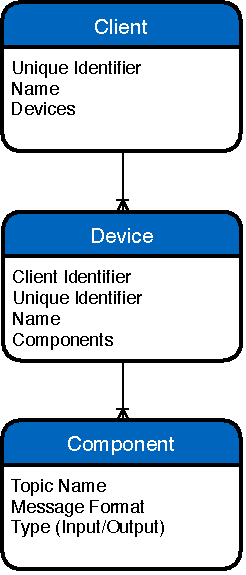
\includegraphics[height=6.5cm]{figures/implementation/ubii_er_client.pdf}
    \caption{The client components.}\label{fig:ubii-er-client}
  \end{subfigure}%
  \begin{subfigure}{.5\textwidth}
    \centering
    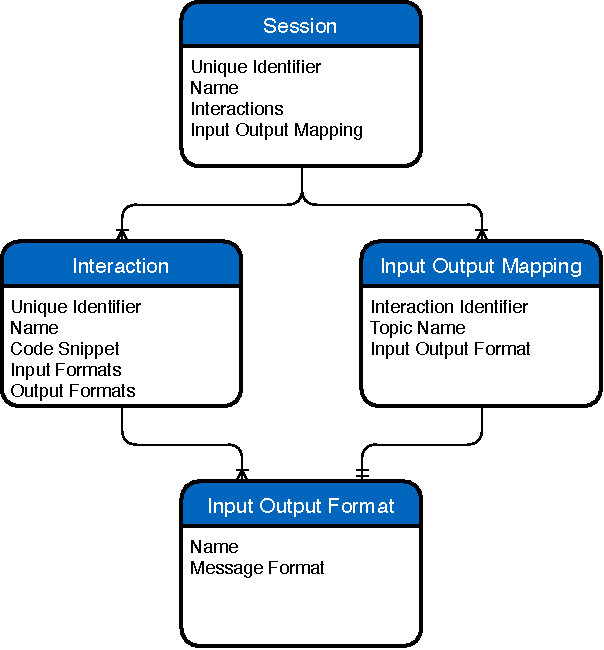
\includegraphics[height=6.5cm]{figures/implementation/ubii_er_server.pdf}
    \caption{The session components.}\label{fig:ubii-er-server}
  \end{subfigure}
  \caption[UBII components diagram]{Relationships of the core components in an entity relationship diagram.}\label{fig:ubii-er}
\end{figure}


\subsection{Interactions}\label{subsection:interactions}
A powerful but optional core feature of \ac{UBII} are interactions. As explained in the component overview~(see~\ref{subsection:architecture}), they are reactive components, which operate on \ac{UBII} topics and regularly execute given code snippets (processing functions) on the \ac{UBII} server. Interactions are isolated components, which just depend on topic data and nothing else. This abstraction introduces the possibility to reuse logic in other applications in a similar context. The data flow from a device to the interaction is visualized in the Figure~\ref{fig:ubii-cd}.

\begin{figure}[htpb]
  \centering
  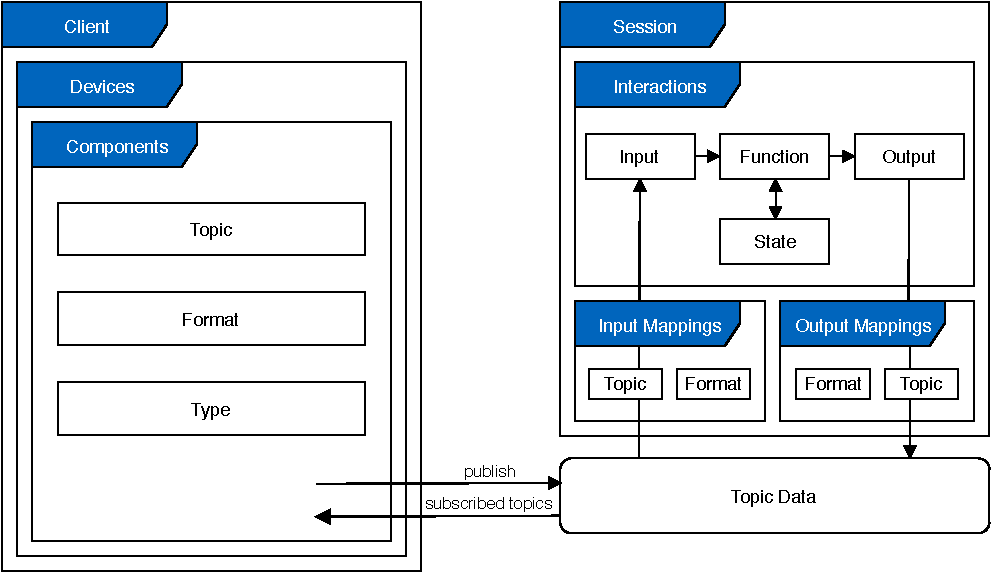
\includegraphics[width=12cm]{figures/implementation/ubii_cd.pdf}
  \caption[UBII communication diagram]{\ac{UBII} interaction processing overview. This graphic gives a rough overview of the dataflow when using an \ac{UBII} interaction. Figure created with the help of Sandro Weber.}\label{fig:ubii-cd}
\end{figure}

\ac{UBII} Interactions should be designed generalized so that they are easy to reuse. They can be used to discretize data, converting data to other formats or just to outsource some logic from the application. Concrete examples include detecting button presses, transforming coordinates and evaluating data. An example implementation which detects position changes can be seen in Figure~\ref{fig:ubii-interaction-example}.

% this might be left out or merged into above
They are also useful if two \ac{UBII} topics with different formats should be connected. An example of such a scenario could be an application, which consumes a rotation given in Euler angles. But some input \ac{UBII} devices publish Euler angles in degrees. A \ac{UBII} interaction, which takes Euler angles in degrees from one \ac{UBII} topic and publishes Euler angles in radians to another one could be implemented.

\begin{figure}[H]
  \begin{lstlisting}[language=JavaScript]
    // detect intentional movement by comparing the current position with a previous one
    function (inputs, outputs, state) {
      const threshold = 0.05;

      if (state.lastPosition) {
        const vector = {
          x: inputs.position.x - state.lastPosition.x,
          y: inputs.position.y - state.lastPosition.y,
        };
  
        const squaredDistance = Math.pow(vector.x, 2) + Math.pow(vector.y, 2);
  
        outputs.moved = squaredDistance < threshold;
      } else {
        outputs.moved = true;
      }

      state.lastPosition = inputs.position;
    }
  \end{lstlisting}
  \caption[Basic UBII interaction in JavaScript]{An example for an \ac{UBII} interaction written in JavaScript. This \ac{UBII} interaction calculates the squared distance of two points. One of the points is provided through the input, while the other one is stored in the state variable. To achieve this, the Euclidean vector norm of the subtraction of both vectors without the square root is calculated and compared with a threshold constant. The result is then written into the output as a boolean data type. This is used to detect intended changes of the input position.}\label{fig:ubii-interaction-example} %TODO: maybe explain as a formula
\end{figure}

The code snippet has to define a function, which accepts three parameters: 
\lstinline{inputs} is a collection of values, which contains values which were published into a \ac{UBII} topic. The \ac{UBII} topic which was used, is defined by the input mappings of the \ac{UBII} session. \lstinline{outputs} is an empty collection, where values can be added. Those values are then published into a \ac{UBII} topic, defined by the output mappings of the \ac{UBII} session. \lstinline{state} stores a persistent collection of values, which can be used in later executions of the same \ac{UBII} interaction.